% !TeX program = XeLaTeX
% !TeX root = ../pujavidhanam.tex
\sect{नवग्रहपूजा}

(चित्रे दर्शितवत् मण्डलानि प्रतिष्ठाप्य आरभेत।)

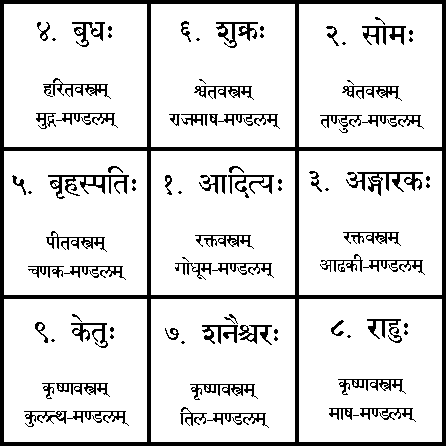
\includegraphics{purvanga/navagraha-diagram.pdf}

\twolineshloka
{जपाकुसुमसङ्काशं काश्यपेयं महद्युतिम्}
{तमोऽरिं सर्वपापघ्नं प्रणतोऽस्मि दिवाकरम्}

आ स॒त्येन॒ रज॑सा॒ वर्त॑मानो निवे॒शय॑न्न॒मृतं॒ मर्त्यं॑ च। हि॒र॒ण्यये॑न सवि॒ता रथे॒नाऽदे॒वो या॑ति॒
भुव॑ना वि॒पश्य\sn{}। अ॒ग्निं दू॒तं वृ॑णीमहे॒ होता॑रं वि॒श्ववे॑दसम्। अ॒स्य य॒ज्ञस्य॑ सु॒क्रतुम्॥
येषा॒मीशे॑ पशु॒पति॑ पशू॒नां चतु॑ष्पदामु॒त च॑ द्वि॒पदाम्। निष्क्री॑तो॒ऽयं य॒ज्ञियं॑ भा॒गमे॑तु
रा॒यस्पोषा॒ यज॑मानस्य सन्तु॥  अधिदेवता प्रत्यधिदेवता सहिताय आदित्याय॒ नम॥ 

अस्मिन् मण्डले अधिदेवता-प्रत्यधिदेवता-सहितं आदित्य-ग्रहं ध्यायामि। आवाहयामि।

\twolineshloka
{दधिशङ्खतुषाराभं क्षीरोदार्णवसम्भवम्}
{नमामि शशिनं सोमं शम्भोर्मुकुटभूषणम्}

आप्या॑यस्व॒ समे॑तु ते वि॒श्वत॑ सोम॒ वृष्णि॑यम्। भवा॒ वाज॑स्य सङ्ग॒थे॥ अ॒प्सु मे॒ सोमो॑
अब्रवीद॒न्तर्विश्वा॑नि भेष॒जा। अ॒ग्निं च॑ वि॒श्वश॑म्भुव॒माप॑श्च वि॒श्वभे॑षजीः। गौ॒री मि॑माय
सलि॒लानि॒ तक्ष॒ती। एक॑पदी द्वि॒पदी॒ सा चतु॑ष्पदी। अ॒ष्टाप॑दी॒ नव॑पदी बभू॒वुषी। स॒हस्राक्षरा पर॒मे
व्यो॑मन्।  अधिदेवता प्रत्यधिदेवता सहिताय सोमाय॒ नम॥ 

अस्मिन् मण्डले अधिदेवता-प्रत्यधिदेवता-सहितं सोम-ग्रहं ध्यायामि। आवाहयामि।


\twolineshloka
{धरणीगर्भसम्भूतं विद्युत्कान्तिसमप्रभम्}
{कुमारं शक्तिहस्तं च मङ्गलं प्रणमाम्यहम्}

अ॒ग्निर्मू॒र्द्धा दि॒वः क॒कुत्पति॑ पृथि॒व्या अ॒यम्। अ॒पा रेतासि जिन्वति। स्यो॒ना पृ॑थिवि॒
भवा॑ऽनृक्ष॒रा नि॒वेश॑नी। यच्छा॑न॒ शर्म॑ स॒प्रथा। क्षेत्र॑स्य॒ पति॑ना व॒य हि॒ते ने॑व जयामसि।
गामश्वं॑ पोषयि॒त्न्वा स नो॑ मृडाती॒दृशे॥  अधिदेवता प्रत्यधिदेवता सहिताय अङ्गारकाय॒ नम॥ 

अस्मिन् मण्डले अधिदेवता-प्रत्यधिदेवता-सहितं अङ्गारक-ग्रहं ध्यायामि। आवाहयामि।


\twolineshloka
{प्रियङ्गुकलिकाश्यामं रूपेणाप्रतिमं बुधम्}
{सौम्यं सौम्यगुणोपेतं तं बुधं प्रणमाम्यहम्}

उद्बु॑ध्यस्वाग्ने॒ प्रति॑जागृह्येनमिष्टापू॒र्ते ससृ॑जेथाम॒यं च॑। पुन॑ कृ॒ण्वस्त्वा॑ पि॒तरं॒
युवा॑नम॒न्वातासी॒त्वयि॒ तन्तु॑मे॒तम्॥ इ॒दं विष्णु॒र्विच॑क्रमे त्रे॒धा निद॑धे प॒दम्। समू॑ढमस्यपा
सु॒रे॥ विष्णो॑ र॒राट॑मसि॒ विष्णो पृ॒ष्ठम॑सि॒ विष्णो॒ श्नप्त्रेस्थो॒ विष्णो॒ स्यूर॑सि॒
विष्णोर्ध्रु॒वम॑सि वैष्ण॒वम॑सि॒ विष्ण॑वे त्वा।  अधिदेवता प्रत्यधिदेवता सहिताय बुधाय॒ नम॥ 

अस्मिन् मण्डले अधिदेवता-प्रत्यधिदेवता-सहितं बुध-ग्रहं ध्यायामि। आवाहयामि।


\twolineshloka
{देवानां च ऋषीणां च गुरुं काञ्चनसन्निभम्}
{बुद्धिभूतं त्रिलोकेशं तं नमामि बृहस्पतिम्}

बृह॑स्पते॒ अति॒यद॒र्यो अर्हाद्वि॒मद्वि॒भाति॒ क्रतु॑म॒ज्जने॑षु। यद्दी॒दय॒च्छव॑सर्त\-प्रजात॒
तद॒स्मासु॒ द्रवि॑णं धेहि चि॒त्रम्॥ इन्द्र॑मरुत्व इ॒ह पा॑हि॒ सोमं॒ यथा॑ शार्या॒ते अपि॑बः सु॒तस्य॑।
तव॒ प्रणी॑ती॒ तव॑ शूर॒शर्म॒न्नावि॑वासन्ति क॒वय॑ सुय॒ज्ञाः॥ ब्रह्म॑जज्ञा॒नं प्र॑थ॒मं
पु॒रस्ता॒द्विसी॑म॒तः सु॒रुचो॑ वे॒न आ॑वः। सबु॒ध्निया॑ उप॒मा अ॑स्य वि॒ष्ठाः स॒तश्च॒ योनि॒मस॑तश्च॒
विव॑॥ अधिदेवता प्रत्यधिदेवता सहिताय बृहस्पतये॒ नम॥ 

अस्मिन् मण्डले अधिदेवता-प्रत्यधिदेवता-सहितं बृहस्पति-ग्रहं ध्यायामि। आवाहयामि।

\twolineshloka
{हिमकुन्दमृणालाभं दैत्यानां परमं गुरुम्}
{सर्वशास्त्रप्रवक्तारं भार्गवं प्रणमाम्यहम्}

प्रव॑ शु॒क्राय॑ भा॒नवे॑ भरध्व ह॒व्यं म॒तिं चा॒ग्नये॒ सुपू॑तम्॥ यो दैव्या॑नि॒ मानु॑षा
ज॒नूष्य॒न्तर्विश्वा॑नि वि॒द्म ना॒ जिगा॑ति॥ इ॒न्द्रा॒णीमा॒सु नारि॑षु सु॒पत्नी॑म॒हम॑श्रवम्। न
ह्य॑स्या अप॒रञ्च॒न ज॒रसा॒ मर॑ते॒ पति॑॥ इन्द्रं॑ वो वि॒श्वत॒स्परि॒ हवा॑महे॒ जनेभ्यः। अ॒स्माक॑मस्तु॒
केव॑लः॥  अधिदेवता प्रत्यधिदेवता सहिताय शुक्राय॒ नम॥ 

अस्मिन् मण्डले अधिदेवता-प्रत्यधिदेवता-सहितं शुक्र-ग्रहं ध्यायामि। आवाहयामि।

\twolineshloka
{नीलाञ्जनसमाभासं रविपुत्रं यमाग्रजम्}
{छायामार्तण्डसम्भूतं तं नमामि शनैश्चरम्}

शं नो॑ दे॒वीर॒भिष्ट॑य॒ आपो॑ भवन्तु पी॒तये। शंयोर॒भिस्र॑वन्तु नः॥ प्रजा॑पते॒ न त्वदे॒तान्य॒न्यो
विश्वा॑ जा॒तानि॒ परि॒ता ब॑भूव। यत्का॑मास्ते जुहु॒मस्तन्नो॑ अस्तु व॒य स्या॑म॒ पत॑यो रयी॒णाम्। इ॒मं
य॑मप्रस्त॒रमाहि सीदाऽङ्गि॑रोभिः पि॒तृभि॑ संविदा॒नः। आत्वा॒ मन्त्रा कविश॒स्ता व॑हन्त्वे॒ना रा॑जन्
ह॒विषा॑ मादयस्व॥  अधिदेवता प्रत्यधिदेवता सहिताय शनैश्चराय॒ नम॥ 

अस्मिन् मण्डले अधिदेवता-प्रत्यधिदेवता-सहितं शनैश्चर-ग्रहं ध्यायामि। आवाहयामि।

\twolineshloka
{अर्धकायं महावीर्यं चन्द्रादित्यविमर्दनम्}
{सिंहिकागर्भसम्भूतं तं राहुं प्रणमाम्यहम्}

कया॑ नश्चि॒त्र आभु॑वदू॒ती स॒दावृ॑ध॒ सखा। कया॒ शचि॑ष्ठया वृ॒ता। आऽयङ्गौः
पृश्नि॑रक्रमी॒दस॑नन्मा॒तरं॒ पुन॑। पि॒तरं॑ च प्र॒यन्त्सुव॑। यत्ते॑ दे॒वी निर्ऋ॑तिराब॒बन्ध॒ दाम॑
ग्री॒वास्व॑विच॒र्त्यम्। इ॒दं  ते॒ तद्विष्या॒म्यायु॑षो॒ न मध्या॒दथा॑जी॒वः पि॒तुम॑द्धि॒ प्रमु॑क्तः॥ 
अधिदेवता प्रत्यधिदेवता सहिताय राहवे॒ नम॥ 

अस्मिन् मण्डले अधिदेवता-प्रत्यधिदेवता-सहितं राहु-ग्रहं ध्यायामि। आवाहयामि।

\twolineshloka
{पलाशपुष्पसङ्काशं तारकाग्रहमस्तकम्}
{रौद्रं रौद्रात्मकं घोरं तं केतुं प्रणमाम्यहम्}

के॒तुं कृ॒ण्वन्न॑के॒तवे॒ पेशो॑ मर्या अपे॒शसे। समु॒षद्भि॑रजायथाः॥ ब्र॒ह्मा दे॒वानां पद॒वीः
क॑वी॒नामृषि॒र्विप्रा॑णां महि॒षो मृ॒गाणाम्। श्ये॒नो गृध्रा॑णा॒ स्वधि॑ति॒र्वना॑ना॒ सोम॑
प॒वित्र॒मत्ये॑ति॒ रेभ\sn{}। (ऋक्) सचि॑त्र चि॒त्रं चि॒तयन् तम॒स्मे चित्र॑क्षत्र चि॒त्रत॑मं वयो॒धाम्।
च॒न्द्रं र॒यिं पु॑रु॒वीरं बृ॒हन्तं॒ चन्द्र॑च॒न्द्राभि॑र्गृण॒ते यु॑वस्व॥  अधिदेवता प्रत्यधिदेवता
सहिताय केतवे॒ नम॥ 

अस्मिन् मण्डले अधिदेवता-प्रत्यधिदेवता-सहितं केतु-ग्रहं ध्यायामि। आवाहयामि।

आदित्यादि नवग्रहदेवताभ्यो नमः आसनं समर्पयामि।
पाद्यं समर्पयामि। अर्घ्यं समर्पयामि। आचमनीयं समर्पयामि। 

शुद्धोदकस्नानं समर्पयामि। स्नानानन्तरम् आचमनीयं समर्पयामि।
वस्त्रार्थम् अक्षतान् समर्पयामि।\\
यज्ञोपवीताभरणार्थे अक्षतान् समर्पयामि।\\
दिव्यपरिमलगन्धान् धारयामि।\\
गन्धस्योपरि हरिद्राकुङ्कुमं समर्पयामि। अक्षतान् समर्पयामि। \\
पुष्पैः पूजयामि।

\begin{enumerate}%[label=\devanumber\value{enumi}]
\item ॐ आदित्याय नमः
\item ॐ अङ्गारकाय नमः
\item ॐ शुक्राय नमः
\item ॐ सोमाय नमः
\item ॐ बुधाय नमः
\item ॐ बृहस्पतये नमः
\item ॐ शनैश्चराय नमः
\item ॐ राहवे नमः
\item ॐ केतवे नमः
\end{enumerate}

नानाविध-परिमल-पत्र-पुष्पाणि समर्पयामि।

आदित्यादि नवग्रहदेवताभ्यो नमः धूपमाघ्रापयामि।\\
दीपं दर्शयामि।\\
नैवेद्यम्। \\
कर्पूरताम्बूलं समर्पयामि। कर्पूरनीराजनं दर्शयामि।\\
प्रार्थनाः समर्पयामि।
अनन्तकोटिप्रदक्षिणनमस्कारान् समर्पयामि।\\

आदित्यादि नवग्रहदेवताभ्यो नमः (अक्षतान् समर्पयित्वा) यथास्थानं प्रतिष्ठापयामि। शोभनार्थे क्षेमाय पुनरागमनाय च।
